The main components of a logic tree structure in the \glsdesc{acr:oqe} are the
following:

\begin{description}

    \item[branch]: the simplest component of a logic tree structure. A branch
	represent a possible interpretation of a value assignment for a specific type
	of uncertainty. It is fully described by the tuple (parameter or model,
	weight).

    \item[branching set]: it is a key component in the logic tree structure
	used by the \gls{acr:oqe}. It groups a set of branches i.e. alternative
	interpretations of a parameter or a model. Each branching set is defined by:

    \begin{itemize}

        \item An ID

        \item An uncertainty type (for a comprehensive list of the types of
		uncertainty currently supported see page~\pageref{list_epistemic_unc})

        \item One or more branches

    \end{itemize}

    This set of uncertainties can be applied to the whole initial  seismic
    source input model or just to a subset of seismic sources. The sum of the
    weights/probabilities assigned to the set  of branches always correspond
    to one.

    \item[branching level]: it is the largest container. It is not used in
	modelling uncertainty, but it is useful in maintaining a logic and an
	order in the structure of the tree.

\end{description}

Below we provide a simple schema illustrating the skeleton of xml file
containing the desciption of a logic tree:

\begin{minted}[firstline=1,firstnumber=1,fontsize=\footnotesize,frame=single,bgcolor=lightgray]{xml}
<logicTreeBranchingLevel branchingLevelID=ID>
    <logicTreeBranchSet branchSetID=ID
                        uncertaintyType=TYPE>
        <logicTreeBranch>
            <uncertaintyModel>VALUE</uncertaintyModel>
            <uncertaintyWeight>WEIGHT</uncertaintyWeight>
        </logicTreeBranch>
    </logicTreeBranchSet>
</logicTreeBranchingLevel>
\end{minted}

As it appears from this example, the structure of a logic tree is a set of
nested elements.

A schematic representation of the elemental components of a logic tree
structure is provided in Figure~\ref{glts}. A branching level identifies the
position where branching occurs while  a branch set identifies a collection of
branches (i.e. individual branches)  whose weights sum to 1.

\begin{figure}[!ht]
\centering
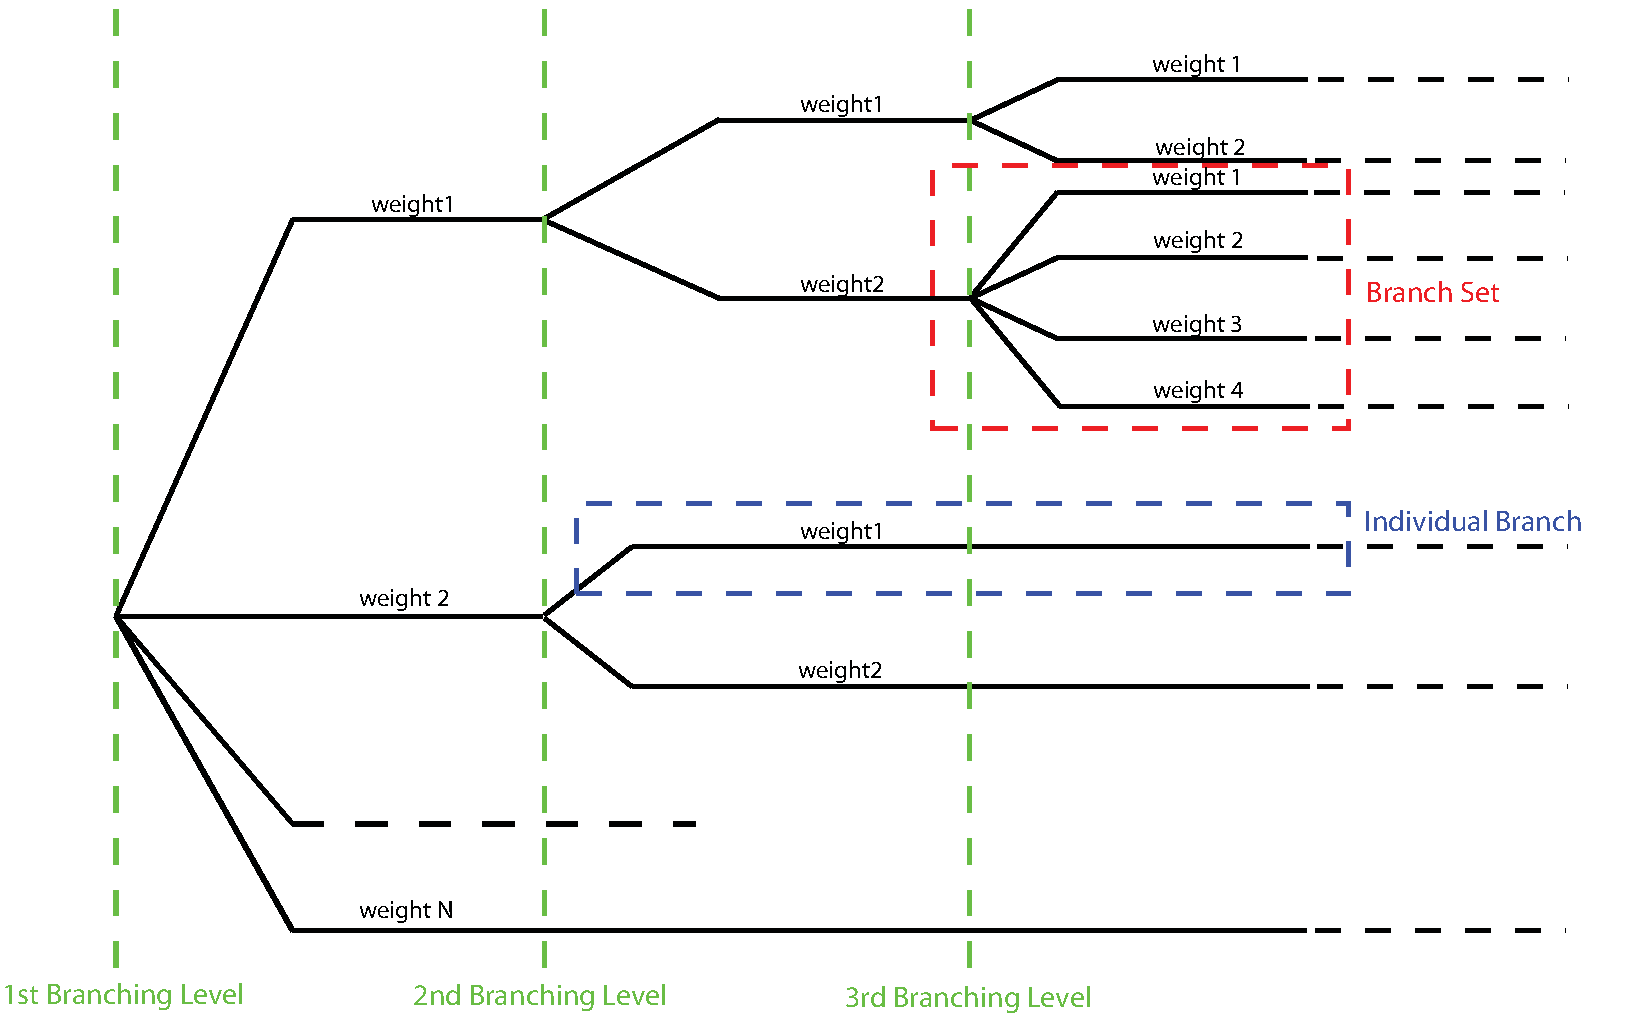
\includegraphics[width=13cm]{figures/hazard/GenericLogicTreeStructure.pdf}
\caption{Generic Logic Tree structure as described in terms of branching
levels, branch sets, and individual branches.}
\label{glts}
\end{figure}

\subsection{Logic trees as described in the nrml schema}

In the NRML schema, a logic tree structure is defined through the
\Verb+logicTree+ element:

\begin{minted}[firstline=1,firstnumber=1,fontsize=\footnotesize,frame=single,bgcolor=lightgray]{xml}
<logicTree logicTreeID="ID">
...
</logicTree>
\end{minted}

A \Verb+logicTree+ contains as a sequence of \Verb+logicTreeBranchingLevel+ elements. The position in the sequence of a \Verb+logicTreeBranchingLevel+ specifies the level of the tree where it is located. That is, the first \texttt{logicTreeBranchingLevel} element in the sequence represents  the first level in the tree, the second element the second level in the tree, and so on.

\begin{minted}[firstline=1,firstnumber=1,fontsize=\footnotesize,frame=single,bgcolor=lightgray]{xml}
<logicTree logicTreeID="ID">
	<logicTreeBranchingLevel branchingLevelID="ID_1">
		...
	</logicTreeBranchingLevel>
	<logicTreeBranchingLevel branchingLevelID="ID_2">
		...
	</logicTreeBranchingLevel>
	....
	<logicTreeBranchingLevel branchingLevelID="ID_N">
		...
	</logicTreeBranchingLevel>
</logicTree>
\end{minted}

There are no restrictions on the number of tree levels that can be defined.

A \Verb+logicTreeBranchingLevel+ is defined as a sequence of
\Verb+logicTreeBranchSet+ elements where each \Verb+logicTreeBranchSet+
defines a particular epistemic uncertainty inside a branching level.

A branch set has two required attributes: \Verb+branchSetID+ and
\Verb+uncertaintyType+. The latter defines the type of epistemic uncertainty this branch set is describing.

\begin{minted}[firstline=1,firstnumber=1,fontsize=\footnotesize,frame=single,bgcolor=lightgray]{xml}
<logicTree logicTreeID="ID">
...
	<logicTreeBranchingLevel branchingLevelID="ID_#">
		<logicTreeBranchSet branchSetID="ID_1"
			uncertaintyType="UNCERTAINTY_TYPE">
			...
		</logicTreeBranchSet>
		<logicTreeBranchSet branchSetID="ID_2"
			uncertaintyType="UNCERTAINTY_TYPE">
			...
		</logicTreeBranchSet>
		...
		<logicTreeBranchSet branchSetID="ID_N"
			uncertaintyType="UNCERTAINTY_TYPE">
			...
		</logicTreeBranchSet>
	</logicTreeBranchingLevel>
...
</logicTree>
\end{minted}

Possible values for the \Verb+uncertaintyType+ attribute are:

\label{list_epistemic_unc}
\begin{itemize}

    \item \Verb+gmpeModel+: indicates epistemic uncertainties on ground
	motion prediction equations

	\item \Verb+sourceModel+: indicates epistemic uncertainties on source models

    \item \Verb+maxMagGRRelative+: indicates relative (i.e. increments)
	epistemic uncertainties to be added (or subtracted, depending on the sign
	of the increment) to the Gutenberg-Richter maximum magnitude value.

    \item \Verb+bGRRelative+: indicates relative epistemic uncertainties
	to be applied to the Gutenberg-Richter b value.

    \item \Verb+abGRAbsolute+: indicates absolute (i.e. values used to replace
	original values) epistemic uncertainties on the Gutenberg-Richter a and b
	values.

    \item \Verb+maxMagGRAbsolute+: indicates (absolute) epistemic
	uncertainties on the Gutenberg-Richter maximum magnitude.
	
	\item \Verb+incrementalMFDAbsolute+: indicates (absolute) epistemic uncertainties on the incremental magnitude frequency distribution (i.e. alternative rates and/or minimum magnitude) of a specific source (can only be applied to individual sources)
	
	\item \Verb+simpleFaultGeometryAbsolute+: indicates alternative representations of the simple fault geometry for an individual simple fault source
	
	\item \Verb+simpleFaultDipRelative+: indicates a relative increase or decrease in fault dip for one or more simple fault sources
	
	\item \Verb+simpleFaultDipAbsolute+: indicates alternative values of fault dip for one or more simple fault sources
	
	\item \Verb+complexFaultGeometryAbsolute+: indicates alternative representations of complex fault geometry for an individual complex fault source

	\item \Verb+characteristicFaultGeometryAbsolute+: indicates alternative representations of the characteristic fault geometry for an individual characteristic fault source

\end{itemize}

There are no restrictions on the number of branch sets that can be defined inside a branching level.

A \Verb+branchSet+ is defined as a sequence of \Verb+logicTreeBranch+
elements, each specified by an \Verb+uncertaintyModel+ element (a string
identifying an uncertainty model; the content of the string varies with the \texttt{uncertaintyType} attribute value of the branchSet element) and the \texttt{uncertaintyWeight} element (specifying the probability/weight associated to the uncertaintyModel):

\begin{minted}[firstline=1,firstnumber=1,fontsize=\footnotesize,frame=single,bgcolor=lightgray]{xml}
< logicTree  logicTreeID="ID">
...
	< logicTreeBranchingLevel  branchingLevelID="ID_#">
		...
		< logicTreeBranchSet  branchSetID="ID_#"
				uncertaintyType="UNCERTAINTY_TYPE">
			< logicTreeBranch  branchID="ID_1">
				<uncertaintyModel>
				    UNCERTAINTY_MODEL
				</uncertaintyModel>
				<uncertaintyWeight>
				    UNCERTAINTY_WEIGHT
				</uncertaintyWeight>
			</ logicTreeBranch >
			...
			< logicTreeBranch  branchID="ID_N">
				<uncertaintyModel>
				    UNCERTAINTY_MODEL
				</uncertaintyModel>
				<uncertaintyWeight>
				    UNCERTAINTY_WEIGHT
				</uncertaintyWeight>
			</logicTreeBranch>
		</logicTreeBranchSet>
		...
	</logicTreeBranchingLevel>
...
</logicTree >
\end{minted}

Depending on the \Verb+uncertaintyType+ the content of the
\Verb+<uncertaintyModel>+ element changes:

\begin{itemize}

    \item if \Verb+uncertaintyType="gmpeModel"+, the uncertainty model
	contains the name of a ground motion prediction equation (a list of
	available GMPEs are given in Appendix~\ref{chap:gsims}), e.g.:

    \begin{minted}[firstline=1,firstnumber=1,fontsize=\footnotesize,frame=single,bgcolor=lightgray]{xml}
<uncertaintyModel>GMPE_NAME</uncertaintyModel>
	\end{minted}

    \item if \Verb+uncertaintyType="sourceModel"+, the uncertainty model
	contains the paths to a source model file, e.g.:

    \begin{minted}[firstline=1,firstnumber=1,fontsize=\footnotesize,frame=single,bgcolor=lightgray]{xml}
<uncertaintyModel>SOURCE_MODEL_FILE_PATH</uncertaintyModel>
	\end{minted}

    \item if \Verb+uncertaintyType="maxMagGRRelative"+, the uncertainty model
	contains the increment to be added (or subtracted, depending on the sign)
	to the Gutenberg-Richter maximum magnitude:

    \begin{minted}[firstline=1,firstnumber=1,fontsize=\footnotesize,frame=single,bgcolor=lightgray]{xml}
<uncertaintyModel>MAX_MAGNITUDE_INCREMENT</uncertaintyModel>
	\end{minted}

    \item if \Verb+uncertaintyType="bGRRelative"+, the uncertainty model
	contains the increment to be added (or subtracted, depending on the sign)
	to the Gutenberg-Richter b value:

    \begin{minted}[firstline=1,firstnumber=1,fontsize=\footnotesize,frame=single,bgcolor=lightgray]{xml}
<uncertaintyModel>B_VALUE_INCREMENT</uncertaintyModel>
	\end{minted}

    \item if \Verb+uncertaintyType="abGRAbsolute"+, the uncertainty model
	must contain one a and b pair:

    \begin{minted}[firstline=1,firstnumber=1,fontsize=\footnotesize,frame=single,bgcolor=lightgray]{xml}
<uncertaintyModel>A_VALUE B_VALUE</uncertaintyModel>
	\end{minted}

    \item if \Verb+uncertaintyType="maxMagGRAbsolute"+, the uncertainty
	model must contain one Gutenberg-Richter maximum magnitude value:

    \begin{minted}[firstline=1,firstnumber=1,fontsize=\footnotesize,frame=single,bgcolor=lightgray]{xml}
<uncertaintyModel>MAX_MAGNITUDE</uncertaintyModel>
	\end{minted}
	
	\item if \Verb+uncertaintyType="incrementalMFDAbsolute"+, the uncertainty model must contain an instance of the incremental MFD node:
	
    \begin{minted}[firstline=1,firstnumber=1,fontsize=\footnotesize,frame=single,bgcolor=lightgray]{xml}
<uncertaintyModel>
    <incrementalMFD
        minMag="MIN MAGNITUDE"
        binWidth="BIN WIDTH">
        <occurRates>RATE_1 RATE_2 ... RATE_N</occurRates>
    </incrementalMFD>
</uncertaintyModel>
    \end{minted}

    \item if \Verb+uncertaintyType="simpleFaultGeometryAbsolute"+ then the uncertainty model must contain a \emph{valid} instance of the \verb+simpleFaultGeometry+ node as described in section \ref{desc_simple_fault}

    \item if \Verb+uncertaintyType="simpleFaultDipRelative"+ then the uncertainty model must specify the number of degrees to increase (positive) or decrease (negative) the fault dip. Note that if this increase results in an adjusted fault dip greater than $90^{\circ}$ or less than $0^{\circ}$ an error will occur.
     
    \begin{minted}[firstline=1,firstnumber=1,fontsize=\footnotesize,frame=single,bgcolor=lightgray]{xml}
<uncertaintyModel>DIP_INCREMENT</uncertaintyModel>
	\end{minted}

	\item if \Verb+uncertaintyType="simpleFaultDipAbsolute"+ then the uncertainty model must specify the dip angle (in degrees)

    \begin{minted}[firstline=1,firstnumber=1,fontsize=\footnotesize,frame=single,bgcolor=lightgray]{xml}
<uncertaintyModel>DIP</uncertaintyModel>
	\end{minted}

    \item if \Verb+uncertaintyType="complexFaultGeometryAbsolute"+ then the uncertainty model must contain a \emph{valid} instance of the \verb+complexFaultGeometry+ source node as described in section \ref{desc_complex_fault}
    
    \item if \Verb+uncertaintyType="characteristicFaultGeometryAbsolute"+ then the uncertainty model must contain a \emph{valid} instance of the \verb+characteristicFaultGeometry+ source node, as described in section \ref{desc_characteristic_fault}
\end{itemize}

There are no restrictions on the number of \Verb+logicTreeBranch+ elements
that can be defined in a \Verb+logicTreeBranchSet+, as long as the uncertainty
weights sum to 1.0.

The \Verb+logicTreeBranchSet+ element offers also a number of optional
attributes allowing for complex tree definitions:

\begin{itemize}

    \item \Verb+applyToBranches+: specifies to which \Verb+logicTreeBranch+
	elements (one or more), in the previous branching level, the branch set
	is linked to. The linking is established by defining the IDs of the
	branches to link to:

	\begin{Verbatim}[commandchars=\\\{\}, samepage=true]
	applyToBranches="branchID1 branchID2 .... branchIDN"
	\end{Verbatim}

    The default is the keyword ALL, which means that a branch set is by
    default linked to all branches in the previous branching level. By
    specifying one or  more branches to which the branch set links to, non-
    symmetric logic trees can be defined.

    \item \Verb+applyToSources+: specifies to which source in a source model
	the uncertainty applies to. Sources are specified in terms of their IDs:

	\begin{Verbatim}[commandchars=\\\{\}, samepage=true]
	applyToSources="srcID1 srcID2 .... srcIDN"
	\end{Verbatim}

    \item \Verb+applyToSourceType+: specifies to which source type the
	uncertainty applies to.  Only one source typology can be defined
	(\Verb+area+, \Verb+point+, \Verb+simpleFault+, \Verb+complexFault+), e.g.:

	\begin{Verbatim}[commandchars=\\\{\}, samepage=true]
	applyToSources="area"
	\end{Verbatim}

    \item \Verb+applyToTectonicRegionType+: specifies to which tectonic
	region type the uncertainty applies to. Only one tectonic region type can
	be defined (\texttt{Active Shallow Crust}, \texttt{Stable
	Shallow Crust}, \texttt{Subduction Interface}, \texttt{Subduction}
	\texttt{IntraSlab}, \texttt{Volcanic}), e.g.:

	\begin{Verbatim}[commandchars=\\\{\}]
	applyToTectonicRegionType="Active Shallow Crust"
	\end{Verbatim}

\end{itemize}